Для определения энергии $\beta$-частиц в работе используется магнитный
спектрометр, схема которого показана на рисунке \ref{img::scheme}.
Электроны испускаются радиоактивным источником и попадают в магнитное поле
катушки, ось которой параллельна $OZ$.
\begin{figure}[h]
  \centering
  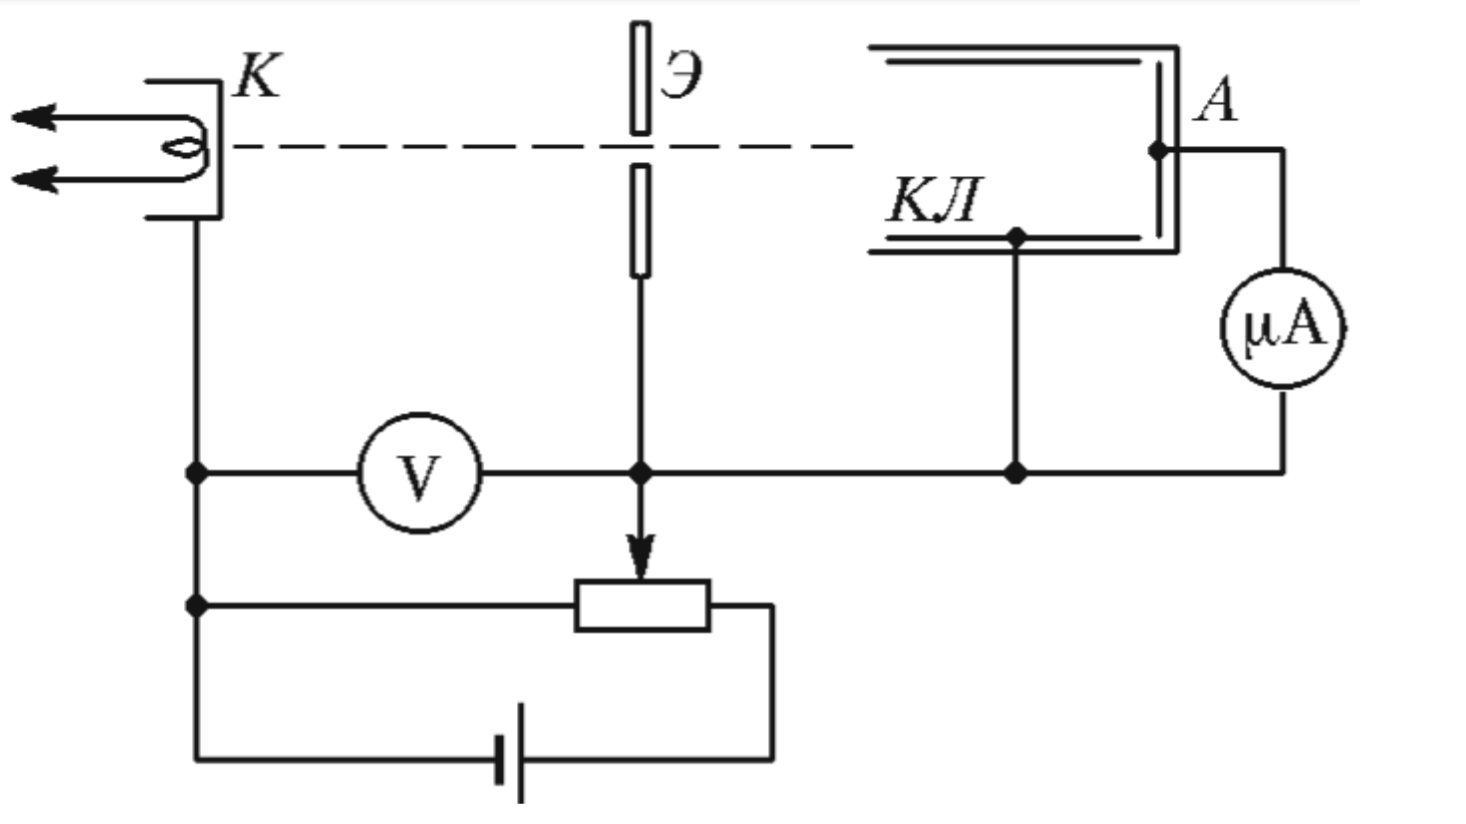
\includegraphics[width=0.7\linewidth]{scheme.png}
  \caption{Схема $\beta$-спектрометра с короткой магнитной линзой.}
  \label{img::scheme}
\end{figure}
Траектории электронов сходятся в одной точке ~---~ фокусе, где и установлен
сцинтилляционный счетчик, сигналы которого усиливаются фотоумножителем и
регистрируются пересчётным прибором. Фокусное расстояние $f$ магнитной линзы
связано с током в катушке $I$ и импульсом $p_e$ регистрируемых частиц следующим
образом:

\[ \frac{1}{f} \propto \frac{I^2}{p_e^2} \]

При неизменной геометрии установки, увеличивая и уменьшая силу тока, можно
фокусировать электроны разных импульсов, причём

\begin{equation}\label{eq::pek}
p_e = kI,
\end{equation}

где $k$ ~---~ коэффициент пропорциональности, являющийся параметром установки.

Блок-схема установки изображена на рисунке \ref{img::block_scheme}.
Радиоактивный источник $^{137}$Cs помещён внутрь откачанной трубы.
Электроны, сфокусированные магнитной линзой, попадают в счётчик.
В газоразрядном счётчике они инициируют газовый разряд и тем
\begin{figure}[h]
  \centering
  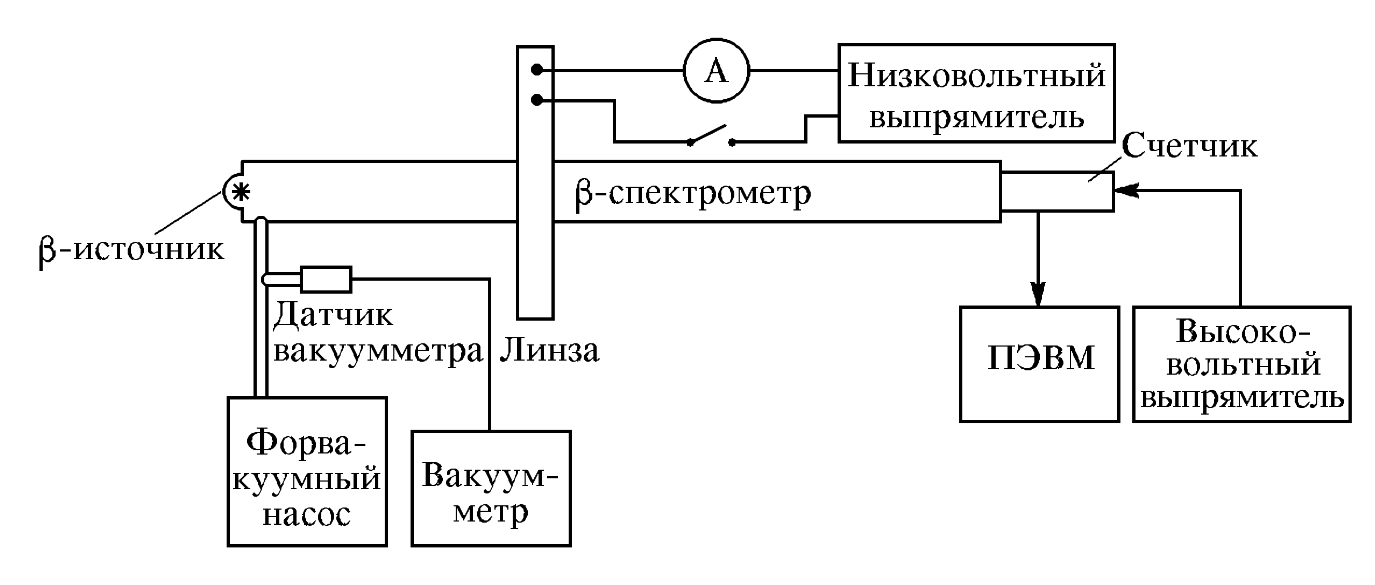
\includegraphics[width=0.7\linewidth]{block_scheme.png}
  \caption{Блок-схема установки для изучения $\beta$-спектра.}
  \label{img::block_scheme}
\end{figure}
самым приводят к появлению электрических импульсов на его электродах, которые
затем регистрируются пересчётным прибором. В результате попадания электронов в
сцинтиллятор на выходе фотоумножителя появляются электрические импульсы, которые
заносятся в память персонального компьютера и выводятся на экран монитора.
Давление в спектрометре поддерживается на уровне около $0.1$ Тор и измеряется
термопарным вакууметром. Лучший вакуум в приборе не нужен, поскольку уже при
этом давлении потери энергии электронов малы и их рассеяние незначительно.
Откачка осуществляется форвакуумным насосом. Магнитная линза питается постоянным
током от выпрямителя. Ток можно повышать до $6$ А, он измеряется цифровым
прибором. Высокое напряжение на ФЭУ или газоразрядный счётчик подаётся от
стабилизированного выпрямителя.